\documentclass[11pt]{article}
\usepackage{acl2012}
\usepackage{times}
\usepackage{latexsym}
\usepackage{amsmath}
\usepackage{multirow}
\usepackage{url}
\usepackage{graphicx}
\usepackage[usenames,dvipsnames]{pstricks}
\usepackage{epsfig}
\DeclareMathOperator*{\argmax}{arg\,max}
\setlength\titlebox{6.5cm}    % Expanding the titlebox

\newcommand{\spectralResult}{59.41}
\newcommand{\collapseResult}{70.82}

\title{A Paradigmatic Model for Learning Syntactic Categories}

\author{First Author \\
  Affiliation / Address line 1 \\
  Affiliation / Address line 2 \\
  Affiliation / Address line 3 \\
  {\tt email@domain} \\\And
  Second Author \\
  Affiliation / Address line 1 \\
  Affiliation / Address line 2 \\
  Affiliation / Address line 3 \\
  {\tt email@domain} \\\And
  Third Author \\
  Affiliation / Address line 1 \\
  Affiliation / Address line 2 \\
  Affiliation / Address line 3 \\
  {\tt email@domain} \\}

\date{}

\begin{document}
\maketitle
\begin{abstract}
We introduce a paradigmatic representation of word context and
demonstrate its utility in learning syntactic categories.  Unlike the
typical syntagmatic representations of word context which consist of
properties of neighboring words, our paradigmatic representation
consists of substitute vectors: possible substitutes of the target
word and their probabilities.  When word contexts are clustered based
on their substitute vectors they reveal a grouping that largely match
the traditional part of speech boundaries with a many-to-one accuracy
of \collapseResult\% on a 45-tag 24K word test corpus.
\end{abstract}

\section{Introduction}
\label{sec:intro}

Grammar rules apply not to individual words (e.g. dog, eat) but to
syntactic categories of words (e.g. noun, verb).  Thus constructing
syntactic categories (also known as lexical or part-of-speech
categories) is one of the fundamental problems in language
acquisition.

Linguists identify syntactic categories based on semantic, syntactic,
and morphological properties of words.  There is also evidence that
children use prosodic and phonological features to bootstrap syntactic
category acquisition \cite{ambridge2011child}.  However there is as
yet no satisfactory computational model that can match human
performance.  Thus identifying the best set of features and best
learning algorithms for syntactic category acquisition is still an
open problem.

Computational models of syntactic category acquisition in the
literature mainly rely on distributional analysis: Items that share
the same distribution (i.e. that occur in the same context) are
grouped into the same category.  The definition of ``the same
context'' vary across studies.  Algorithms based on the Hidden Markov
Model use class based n-grams to specify context
\cite{Brown:1992:CNG:176313.176316}, others use a frame of neighboring
words around the target word \cite{Schutze:1995:DPT:976973.976994}.
Our main contribution in this study is to introduce paradigmatic
features, i.e. features based on potential substitutes of the target
word, to represent word context.

Relationships between linguistic units can be classified into two
types: syntagmatic (concerning positioning), and paradigmatic
(concerning substitution).  Syntagmatic relations determine which
units can combine to create larger groups and paradigmatic relations
determine which units can be substituted for one another.
Figure~\ref{fig:paradigmatic} illustrates the paradigmatic vs
syntagmatic axes for words in a simple sentence and their possible
substitutes.

\begin{figure}[h] \centering
% Generated with LaTeXDraw 2.0.8
% Tue Jan 10 15:57:06 EET 2012
% \usepackage[usenames,dvipsnames]{pstricks}
% \usepackage{epsfig}
% \usepackage{pst-grad} % For gradients
% \usepackage{pst-plot} % For axes
\scalebox{1} % Change this value to rescale the drawing.
{
\begin{pspicture}(0,-1.6728125)(4.73474,1.6528125)
\usefont{T1}{ptm}{m}{n}
\rput(0.39520833,-0.6571875){\psframebox[linewidth=0.04]{the}}
\usefont{T1}{ptm}{m}{n}
\rput(1.8816146,-0.6571875){\psframebox[linewidth=0.04]{man}}
\usefont{T1}{ptm}{m}{n}
\rput(1.9886458,0.3428125){\psframebox[linewidth=0.04,linestyle=dashed,dash=0.16cm 0.16cm]{girl}}
\usefont{T1}{ptm}{m}{n}
\rput(3.3298957,-0.6571875){\psframebox[linewidth=0.04]{cried}}
\usefont{T1}{ptm}{m}{n}
\rput(3.2798958,0.3428125){\psframebox[linewidth=0.04,linestyle=dashed,dash=0.16cm 0.16cm]{died}}
\usefont{T1}{ptm}{m}{n}
\rput(3.3158333,1.3428125){\psframebox[linewidth=0.04,linestyle=dashed,dash=0.16cm 0.16cm]{sang}}
\usefont{T1}{pcr}{m}{n}
\rput(2.020677,-1.4671875){\footnotesize syntagmatic axis}
\usefont{T1}{pcr}{m}{n}
\rput{-90.0}(4.4150524,4.661927){\rput(4.507552,0.1328125){\footnotesize paradigmatic axis}}
\psline[linewidth=0.04cm,arrowsize=0.05291667cm 2.0,arrowlength=1.4,arrowinset=0.4]{<->}(0.13364583,-1.1671875)(3.9336457,-1.1671875)
\psline[linewidth=0.04cm,arrowsize=0.05291667cm 2.0,arrowlength=1.4,arrowinset=0.4]{<->}(4.133646,1.6328125)(4.133646,-1.1671875)
\psline[linewidth=0.04cm](0.81364584,-0.6671875)(1.4136459,-0.6671875)
\psline[linewidth=0.04cm](2.3936458,-0.6671875)(2.8136458,-0.6671875)
\psline[linewidth=0.04cm](1.9136459,0.0528125)(1.9136459,-0.4271875)
\psline[linewidth=0.04cm](3.3136458,0.0928125)(3.3136458,-0.3671875)
\psline[linewidth=0.04cm](3.3136458,1.0128125)(3.3136458,0.6328125)
\end{pspicture} 
}

\caption{Syntagmatic vs. paradigmatic axes for words in a simple
  sentence \cite{chandler2007semiotics}.}
\label{fig:paradigmatic}
\end{figure}

Both syntagmatic and paradigmatic relations of a word can be used to
represent its context.  In the syntagmatic case the context is
represented by a selection of neighboring words, in the paradigmatic
case it is represented by a set of possible substitutes.  In previous
studies of syntactic category learning the context representation has
been primarily syntagmatic, either implicit in the class based n-grams
of the standard Hidden Markov Model, or explicit in the construction
and clustering of left and right neighbors.

In this study we explore a paradigmatic representation of the context
of a word in syntactic category acquisition.  Specifically, the
context of a word is represented by a list of its possible substitutes
and their probabilities, which we call the {\em substitute vector}.
Note that the substitute vector is a function of the context only, not
the target word.  Thus in effect we are clustering contexts, not
words.  When word contexts are clustered based on their substitute
vectors they reveal a grouping that largely match the traditional part
of speech boundaries (\collapseResult\% many-to-one score using a
45-tag 24K word test corpus).
% standard HMM-EM gives 42\% on the same data.

Section~\ref{sec:related} gives a detailed review of related work.
The construction of the substitute vectors is described in
Section~\ref{sec:lm}.  To find out how to best make use of this new
paradigmatic representation, we explore different distance metrics
(Section~\ref{sec:dist}), dimensionality reduction methods
(Section~\ref{sec:dimreduce}), and clustering algorithms
(Section~\ref{sec:clustering}) for substitute vectors.  We note that
close to 95\% of the word occurrences in human labeled data are tagged
with their most frequent part of speech
\cite{Lee:2010:STU:1870658.1870741}, making one-tag-per-word a fairly
good first approximation.  Even ambicategory words generally have
fairly skewed part of speech distributions.
Section~\ref{sec:sparsity} looks at ways to increase the sparsity of
our solutions and demonstrates significant improvements using the
one-tag-per-word assumption and similarity metrics that introduce
sparsity.  Section~\ref{sec:discussion} discusses the results and
Section~\ref{sec:contrib} summarizes our contributions.


\section{Related Work}
\label{sec:related}

There are several good reviews of algorithms for unsupervised
part-of-speech induction
\cite{Christodoulopoulos:2010:TDU:1870658.1870714,Gao:2008:CBE:1613715.1613761}
and models of syntactic category acquisition \cite{ambridge2011child}.
In this review we focus on (i) the information captured by the inputs,
and (ii) the constraints applied to the outputs of the algorithms.

This work is to be distinguished from supervised part-of-speech
disambiguation systems, which use labeled training data
\cite{Church:1988:SPP:974235.974260}, unsupervised disambiguation
systems, which use a dictionary of possible tags for each word
\cite{Merialdo:1994:TET:972525.972526}, or prototype driven systems
which use a small set of prototypes for each class
\cite{Haghighi:2006:PLS:1220835.1220876}.  The problem of induction is
important for studying under-resourced languages that lack labeled
corpora and high quality dictionaries.  It is also essential in
modeling child language acquisition because every child manages to
induce syntactic categories without access to labeled sentences,
labeled prototypes, or dictionary constraints.

\paragraph{Clustering vs. HMMs:}
Models of unsupervised induction of part-of-speech categories fall
into two broad groups.  The first group uses algorithms that cluster
word types based on their context statistics
\cite{Schutze:1995:DPT:976973.976994}.  Work in modeling child
syntactic category acquisition has generally followed this clustering
approach \cite{redington1998distributional,mintz2003frequent}.  The
second group consists of probabilistic models based on the Hidden
Markov Model (HMM) framework \cite{Brown:1992:CNG:176313.176316}.

\paragraph{Clustering and data sparsity:}
Clustering based methods represent context using neighboring words,
typically a single word on the left and a single word on the right
called a ``frame'' (e.g., {\em {\bf the} dog {\bf is}; {\bf the} cat
  {\bf is}}).  They cluster word types rather than word tokens based
on the frames they occupy thus employing one-tag-per-word assumption
from the beginning (with the exception of some methods in
\cite{Schutze:1995:DPT:976973.976994}).  They may suffer from data
sparsity caused by infrequent words and infrequent contexts.  The
solutions suggested either restrict the set of words and set of
contexts to be clustered to the most frequently observed or use
dimensionality reduction.  \cite{redington1998distributional} defines
context similarity based on the number of common frames bypassing the
data sparsity problem but achieves mediocre results.
\cite{mintz2003frequent} only uses the most frequent 45 frames and
\cite{biemann2006unsupervised} clusters the most frequent 10,000 words
using contexts formed from the most frequent 150-200 words.
\cite{Schutze:1995:DPT:976973.976994,lamar-EtAl:2010:Short} employ SVD
to enhance similarity between less frequently observed words and
contexts.  \cite{Lamar:2010:LCU:1870658.1870736} represents each
context by the currently assigned left and right tag (which eliminates
data sparsity) and clusters word types using a soft k-means style
iterative algorithm.  They report the best clustering result to date
of 70.8\% many-to-one accuracy on a 45-tag 1M word corpus.

% all except schutze cluster word types

\paragraph{HMMs and distribution sparsity:}
The prototypical bitag HMM model maximizes the likelihood of the
corpus $w_1 \ldots w_n$ expressed as $P(w_1|c_1)\prod_{i=2}^n
P(w_i|c_i) P(c_i|c_{i-1})$ where $w_i$ are the word tokens and $c_i$
are their (hidden) tags.  One problem with such a model is its
tendency to distribute probabilities equally and the resulting
inability to model highly skewed word-tag distributions observed in
hand-labeled data \cite{johnson:2007:EMNLP-CoNLL2007}.  To favor
sparse word-tag distributions one can enforce a strict
one-tag-per-word solution
\cite{Brown:1992:CNG:176313.176316,Clark:2003:CDM:1067807.1067817},
use sparse priors in a Bayesian setting
\cite{goldwater-griffiths:2007:ACLMain,johnson:2007:EMNLP-CoNLL2007},
or use posterior regularization
\cite{Ganchev:2010:PRS:1859890.1859918}.  Each of these techniques
provide significant improvements over the standard HMM model: for
example \cite{Gao:2008:CBE:1613715.1613761} shows that sparse priors
can gain from 4\% (62\% to 66\% with a 1M word corpus) to 30\% (28\%
to 58\% with a 24K word corpus) in cross-validated many-to-one
accuracy.  However \cite{Christodoulopoulos:2010:TDU:1870658.1870714}
shows that the older one-tag-per-word models such as
\cite{Brown:1992:CNG:176313.176316} outperform the more sophisticated
sparse prior and posterior regularization methods both in speed and
accuracy (the Brown model gets 68\% many-to-one accuracy with a 1M
word corpus).  Given that close to 95\% of the word occurrences in
human labeled data are tagged with their most frequent part of speech
\cite{Lee:2010:STU:1870658.1870741}, this is probably not surprising;
one-tag-per-word is a fairly good first approximation for induction.

\paragraph{Poverty of features:}
Another problem with the plain HMM model is the poverty of its input
features.  Of the syntactic, semantic, and morphological information
linguists claim underlie syntactic categories, bitag HMMs only
represent limited syntactic information in their class based n-grams.
\cite{Clark:2003:CDM:1067807.1067817,bergkirkpatrick-klein:2010:ACL,blunsom-cohn:2011:ACL-HLT2011}
incorporate similar orthographic features and report improvements of
3, 7, and 10\% respectively over the baseline Brown model.
\cite{Christodoulopoulos:2010:TDU:1870658.1870714} use prototype based
features as described in \cite{Haghighi:2006:PLS:1220835.1220876} with
automatically induced prototypes and report an 8\% improvement over
the baseline Brown model.  Semantic information is incorporated to
some extent by some clustering based models and our paradigmatic
model.  To our knowledge, nobody has yet tried to incorporate
phonological or prosodic features in a computational model for
syntactic category acquisition.

\paragraph{Evaluation:}
It is natural to question the merit of evaluating unsupervised results
by comparing them to gold standard tags.  For example
\cite{freudenthal2005resolution} argue that a verb category (such as
{\sc vb} in Penn Treebank) that contains verbs that can and cannot be
used in certain constructions (e.g. the imperative) and verbs that can
be used as both auxiliaries and main verbs (e.g., {\em do, have}) does
not in fact constitute a set of items that could be substituted for
one another in particular sentences.  Such a category fails the
standard linguistic definition of a syntactic category and children do
not seem to make errors of substituting such words in utterances
(e.g. {\em''What do you want?''} vs. {\em *''What put you want?''}).
They suggest evaluating models by incorporating a production component
that allows the model's output to be compared to speech produced by
children exposed to the same input.  \cite{frank2009evaluating},
motivated by the lack of gold standards for many novel languages,
suggest comparing a system's clusters to a set of clusters created
from {\em substitutable frames}.  They create frames using two words
appearing in the corpus with exactly one word between and calculate
precision, recall, and F-score of the system's clustering.
Statistical parsers or factored machine learning systems could also be
sources of extrinsic evaluation for induced syntactic categories.  We
hope such extrinsic evaluation will be more widespread in the future
but nevertheless use the 45-tag Penn Treebank gold standard to
evaluate the current work.

\paragraph{Our work:}
Our work is more closely related to clustering based methods with two
important differences: (i) we represent word contexts not by an ad-hoc
selection of syntagmatic features based on a single word neighborhood
but by substitute vectors defined by a statistical language model
representing paradigmatic features of a larger window, (ii) we cluster
word tokens (or rather their contexts) instead of word types, which
means not being constrained by the one-tag-per-word assumption from
the beginning.  The features in our model incorporate semantic as well
as syntactic information from the context as illustrated by the
examples in Section~\ref{sec:lm}.  Our best results on the 45-tag 24K
corpus given in Section~\ref{sec:sparsity} (\collapseResult\% many-to-one)
compare favorably with best previously reported results on the same
corpus (58.2\% in \cite{Gao:2008:CBE:1613715.1613761}).  This
significant improvement is due to the additional information obtained
from the statistical language model which also comes at a great
computational cost.  Developing faster algorithms to find high
probability substitutes is in our current research agenda.

\section{Substitute Vectors}
\label{sec:lm}

In this study, we predict the part of speech of a word in a given
context based on its substitute vector.  The dimensions of the
substitute vector represent words in the vocabulary, and the entries
in the substitute vector represent the probability of those words
being used in the given context substituting the target word.  This
section details the choice of the data set, the vocabulary and the
estimation of substitute probabilities.

% what is the test data
The first 24,020 tokens of the Penn Treebank \cite{treebank3} Wall
Street Journal Section 00 was used as the test corpus.
% what is the tag set
The treebank uses 45 part-of-speech tags which is the set we used as
the gold standard for comparison in our experiments.
% what is the LM training data
%Train => 5181717 126019973 690121813
To compute substitute probabilities we trained a language model using
approximately 126 million tokens of Wall Street Journal data
(1987-1994) extracted from CSR-III Text \cite{csr3text} (we excluded
the test corpus).
% how is the language model trained
We used SRILM \cite{Stolcke2002} to build a 4-gram language model with
Kneser-Ney discounting.
% what is the vocabulary
Words that were observed less than 500 times in the LM training data
were replaced by \textsc{unk} tags, which gave us a vocabulary size of
12,672.  
% perplexity
The perplexity of the 4-gram language model on the test corpus was
55.4 which is quite low due to using in-domain data and a small
vocabulary.

% how are the substitutes computed
We used both left and right neigbors to estimate the probabilities for
potential substitutes of word $w$ in a context $c_w$.  We define $c_w$
as the $2n-1$ word window centered around the target word position:
$w_{-n+1} \ldots w_0 \ldots w_{n-1}$ ($n=4$ is the LM order).  The
probability of a substitute word in a given context can be estimated
as:
\begin{eqnarray}
  \label{eq:lm1}P(w_0 = w | c_w) & \propto & P(w_{-n+1}\ldots w_0\ldots w_{n-1})\\
  \label{eq:lm2}& = & P(w_{-n+1})P(w_{-n+2}|w_{-n+1})\nonumber\\
  &&\ldots P(w_{n-1}|w_{-n+1}^{n-2})\\
  \label{eq:lm3}& \approx & P(w_0| w_{-n+1}^{-1})P(w_{1}|w_{-n+2}^0)\nonumber\\
  &&\ldots P(w_{n-1}|w_0^{n-2})
\end{eqnarray}
where $w_i^j$ represents the sequence of words $w_i w_{i+1} \ldots
w_{j}$.  In Equation \ref{eq:lm1}, $P(w|c_w)$ is proportional to
$P(w_{-n+1}\ldots w_0 \ldots w_{n+1})$ because the words of the
context are fixed.  Terms without $w_0$ are identical for each
substitute in Equation \ref{eq:lm2} therefore they have been dropped
in Equation \ref{eq:lm3}.  Finally, because of the Markov property of
n-gram language model, only the closest $n-1$ words are used in the
final conditional probability terms.

After computing the unnormalized probability of each of the 12,672
vocabulary words at each of the 24,020 positions in the test corpus
based on Equation~\ref{eq:lm3}, the probability vectors for each
position were normalized to add up to 1.0 giving us the final
substitute vectors used in the rest of this study.  Computation of
substitute vectors is computationally expensive and we are
investigating algorithmic methods that will provide the most likely
substitutes for each position without going through the whole
vocabulary.  However, the focus of this work is to first demonstrate
the usefulness of the substitute vector representation in learning
syntactic categories.

% example substitute vectors (both syntactic and semantic)
The high probability substitutes reflect both semantic and syntactic
features of the context as seen in the examples given in
Table~\ref{tab:subs}.  Top substitutes for the word ``the'' consist of
words that can act as determiners.  Top substitutes for ``board'' are
not only nouns, but specifically nouns compatible with the semantic
context.

\begin{table}[h]\centering
\begin{tabular}{|l|ll|} \hline
% \multicolumn{3}{|l|}
\emph{word} & \emph{substitute} & \emph{probability} \\ \hline
the	& its & .9011 \\
	& the & .0978 \\
	& a & .0007 \\ \hline
board	& company & .5573 \\
	& firm & .2219 \\
	& bank & .0727 \\ \hline
\end{tabular}
\caption{Example substitutes for ``the'' and ``board'' in the sentence {\em ``Pierre Vinken, 61 years old, will join the  board as a nonexecutive director Nov. 29.''}}
\label{tab:subs}
\end{table}

These examples illustrate two concerns inherent in all distributional
methods: (i) words that are generally substitutable like ``the'' and
``its'' are placed in separate categories ({\sc dt} and {\sc prp\$})
by the gold standard, (ii) words that are generally not substitutable
like ``board'' and ``banana'' are placed in the same category ({\sc
  nn}).  Whether gold standard part-of-speech tags or distributional
categories are better suited to applications like parsing or machine
translation can be best decided using extrinsic evaluation.  However
in this study we follow most previous work and evaluate our results by
comparing them to gold standard part-of-speech tags.

\section{Distance Metric}
\label{sec:dist}

We represent each context with a high dimensional probability vector
called the substitute vector as described in the previous section.  In
this section we compare various distance metrics in this high
dimensional space with the goal of discovering one that will judge
vectors that belong to the same syntactic category similar and vectors
that belong to different syntactic categories distant.  The distance
metrics we have considered are listed in Table~\ref{tab:metrics}.

\begin{table}[ht] \centering
\small
\begin{tabular}{|lll|}
\hline
Cosine($\mathbf{p}, \mathbf{q}$) & = & $<\mathbf{p},\mathbf{q}> / (\|\mathbf{p}\|_{2} \|\mathbf{q}\|_{2})$ \\
Euclid($\mathbf{p}, \mathbf{q}$) & = & $\|\mathbf{p} - \mathbf{q}\|_{2}$ \\
Manhattan($\mathbf{p}, \mathbf{q}$) & = & $\|\mathbf{p} - \mathbf{q}\|_{1}$ \\
Maximum($\mathbf{p}, \mathbf{q}$) & = & $\|\mathbf{p} - \mathbf{q}\|_{\infty}$ \\
KL2($\mathbf{p}, \mathbf{q}$) & = & $\sum_i p_iln(p_i/q_i) + q_iln(q_i/p_i) $\\
JS($\mathbf{p}, \mathbf{q}$) & = & $\sum_i p_iln(p_i/m_i) + q_iln(q_i/m_i) $\\
& & where $m_i = (p_i + q_i) / 2$\\
\hline
\end{tabular}
\caption{Similarity metrics.  JS is the Jensen-Shannon divergence and
  KL2 is a symmetric implementation of Kullback-Leibler divergence.}
\label{tab:metrics}
\end{table}

To judge the merit of each distance metric we obtained supervised
baseline scores using leave-one-out cross validation and the weighted
k-nearest-neighbor algorithm\footnote{Neighbors were weighted using
  1/distance, $k=30$ was chosen empirically.} on the gold tags of the
test corpus.  The results are listed in Table~\ref{tab:distscores}
sorted by score.  

\begin{table}[ht] \centering
\begin{tabular}{|l|c|}
\hline
Metric & Accuracy(\%) \\
\hline
KL2 & 0.6889 \\
Manhattan & 0.6865 \\
Jensen & 0.6801 \\
Cosine & 0.6706 \\
Maximum & 0.6663 \\
Euclid & 0.6255 \\
lg2-Maximum & 0.5361 \\
lg2-Cosine & 0.4847 \\
lg2-Euclid & 0.4038 \\
lg2-Manhattan & 0.3729 \\
\hline
\end{tabular}
\caption{Supervised baseline scores with different distance metrics.
  Log-metric indicates that metric applied to the log of the
  probability vectors.}
\label{tab:distscores}
\end{table}

% K=30
% KL2 0.688884263114072
% Manhattan 0.686511240632806
% Jensen 0.680099916736053
% Cosine 0.670566194837635
% Maximum 0.666278101582015
% Euclid 0.625478767693589
% lg2-Maximum 0.536136552872606
% lg2-Cosine 0.484721065778518
% lg2-Euclid 0.403788509575354
% lg2-Manhattan 0.37285595337219

% K=20
% KL2 & 68.95\\
% Manhattan & 68.75\\
% Jensen & 68.43\\
% Cosine & 67.45\\
% Maximum	& 66.55\\
% Euclid & 63.33\\
% log-Maximum & 54.20\\
% log-Cosine & 49.33\\
% log-Euclid & 41.21\\
% log-Manhattan & 37.59\\

The entries with the log- prefix indicate a metric applied to the log
of the probability vectors.  Distance metrics on log probability
vectors performed poorly compared to their regular counterparts
indicating differences in low probability words are relatively
unimportant and high probability substitutes determine syntactic
category.  The surprisingly good result achieved by the simple Maximum
metric (which identifies the dimension with the largest difference
between two vectors) also support this conclusion.  The maximum score
of 69\% can be taken as a rough upper bound for an unsupervised
learner using this space on the 45-tag 24K test corpus because 31\% of
the instances are assigned to the wrong part of speech by the majority
of their closest neighbors.  We will discuss ways to push this upper
bound higher by including other features in
Section~\ref{sec:sparsity}.

% moreover we are using probability vectors so its more natural to use
% kl2

\section{Dimensionality Reduction}
\label{sec:dimreduce}

Using high dimensional vectors is problematic with many learning
algorithms because of computational cost and the curse of
dimensionality.  In this section we investigate if there is a low
dimensional representation of the substitute vectors which still
preserve the neighborhood information necessary to learn syntactic
categories.  We first briefly describe then report experimental
results on principal components analysis (PCA), Isomap
\cite{tenenbaum2000global}, locally linear embedding (LLE)
\cite{roweis2000nonlinear}, and Laplacian eigenmaps
\cite{belkin2003laplacian}.  

Each dimensionality reduction algorithm tries to preserve certain
aspects of the original vectors.  PCA is a linear method that
minimizes reconstruction error.  Isomap tries to preserve distances as
measured along a low dimensional submanifold assuming the input
vectors were sampled from the neighborhood of such a manifold.  LLE
most faithfully preserves the local linear structure of nearby input
vectors.  Laplacian eigenmaps most faithfully preserve proximity
relations, mapping nearby inputs to nearby outputs.

We wanted to see how accuracy (based on the k-nearest-neighbor
supervised baseline as in the previous section) changed based on the
number of dimensions for each dimensionality reduction algorithm.  All
other parameters were set empirically to values that gave reasonable
results: For algorithms that require a distance matrix rather than raw
input vectors we used the KL2 distance judged best by the experiments
of the previous section.  For graph based methods we built
neighborhood graphs using 100 nearest neighbors.  The low dimensional
output vectors were compared using the cosine distance metric for the
supervised k-nearest-neighbor algorithm.  Figure~\ref{fig:dimreduce}
plots supervised baseline accuracy vs. number of dimensions for each
algorithm.

% graph of dims vs accuracy
\begin{figure}[h]
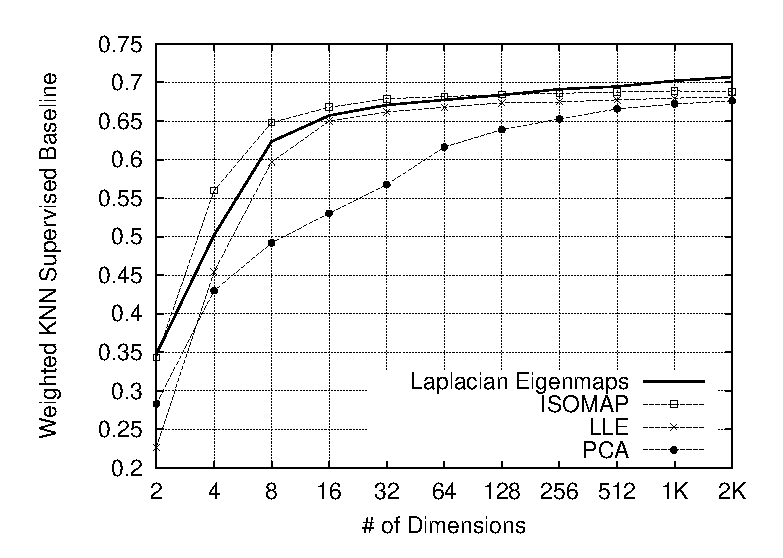
\includegraphics[width=.5\textwidth]{baseline_graph_mono.eps}
\caption{Supervised knn baselines for the four dimensionality
  reduction algorithms.}
\label{fig:dimreduce}
\end{figure}

% /scratch/esert/pos_ind/work/BASELINE_GRAPH/plot_data
% dimension PCA    LLE     ISO     LEM(Spectral)
% 2              0.2831 0.2272 0.3433 0.3480
% 4              0.4300 0.4547 0.5596 0.5019
% 8              0.4920 0.5968 0.6480 0.6234
% 16            0.5303 0.6500 0.6678 0.6572
% 32            0.5676 0.6617 0.6790 0.6708
% 64            0.6162 0.6680 0.6818 0.6774
% 128          0.6390 0.6735 0.6844 0.6838
% 256          0.6527 0.6747 0.6860 0.6914
% 512          0.6658 0.6774 0.6876 0.6948
% 1024        0.6720 0.6798 0.6891 0.7022
% 2048        0.6764 0.6811 0.6878 0.7070
% 

The graph based algorithms (Isomap, LLE, and Laplacian eigenmaps) all
outperform PCA.  They stay within 5\% of their peak accuracy with as
few as 16 dimensions.  In fact Laplacian eigenmaps outperform the
baseline with the original 12,672 dimensional vectors (68.95\%) when
allowed to retain more than about 250 dimensions.  Spectral clustering
uses the same transformation as the Laplacian eigenmaps algorithm and
we compare its performance to other clustering algorithms in the next
section.

\section{Clustering}
\label{sec:clustering}

We compared three clustering algorithms applied to the original
substitute vectors using many-to-one accuracy on the 45-tag 24K word
test corpus.  Hierarchical agglomerative clustering with complete
linkage (HAC) starts with each instance in its own cluster and
iteratively combines the two closest groups (measured by their most
distant points) at each step \cite{manning2008introduction}.
K-medoids minimizes sum of pairwise distances between each datapoint
to the exemplar at the center of its cluster
\cite{kaufman2005finding}.  Spectral clustering\footnote{We used the
  implementation in \cite{chen2011parallel} with a symmetric sparse
  affinity matrix of 550 nearest neighbors.} uses the eigenvalues of
the graph Laplacian $L=D^{-1/2} W D^{-1/2}$ to reduce the number of
dimensions (similar to Laplacian eigenmaps) and uses simple k-means
clustering on the resulting representation \cite{ng2002spectral}.  All
three algorithms accept the distance matrix based on the KL2 distance
(see Section~\ref{sec:dist}) as input.

\begin{figure}[h]
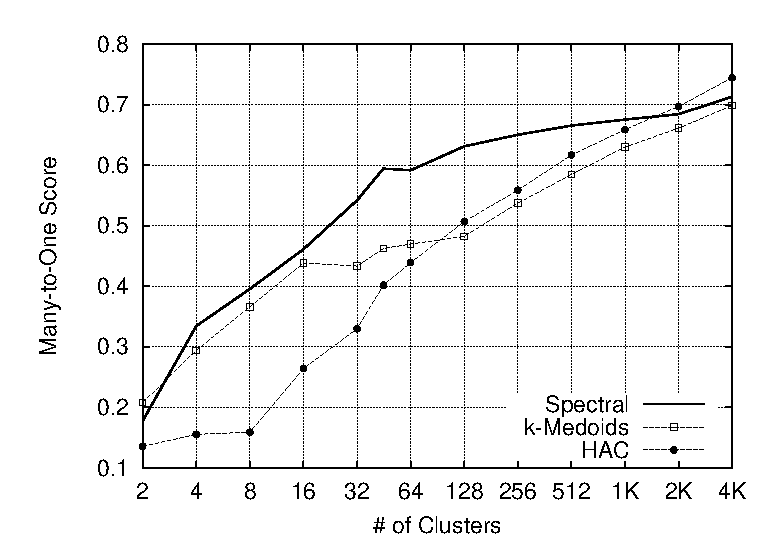
\includegraphics[width=.5\textwidth]{clustering_graph_mono.eps}
\caption{Many-to-one score for three clustering algorithms on the
  45-tag 24K word corpus.}
\label{fig:clustering}
\end{figure}

% #cluster kmedoid spectral hac
% 2          0.20795 0.17781 0.135762
% 4          0.29413 0.33439 0.155579
% 8          0.36615 0.39550 0.159076
% 16        0.43830 0.46116 0.263988
% 32        0.43318 0.54192 0.329850
% 45        0.46245 0.59413 0.401832
% 64        0.46965 0.59151 0.438843
% 128      0.48235 0.63106 0.506703
% 256      0.53709 0.65000 0.558659
% 512      0.58464 0.66520 0.616653
% 1024     0.62985 0.67523 0.658576
% 2048     0.66107 0.68414 0.696878
% 4096     0.69842 0.71286 0.744338


Figure~\ref{fig:clustering} plots the many-to-one score versus number
of clusters for the three algorithms on the 45-tag 24K word test
corpus.  The many-to-one score naturally increases as we approach the
one cluster per word limit, however we find the evolution of the
curves informative.  At the high end (more than 2000 clusters) HAC
performs best with its conservative clusters, but its performance
degrades fast as we reduce the number of clusters because it cannot
reverse the accumulating mistakes.  At the low end (less than 16
clusters) k-medoids and spectral have similar performance.  However
for the region of interest (between 16 to 2000 clusters) spectral
clustering is clearly superior with \spectralResult\% many-to-one
accuracy at 45 clusters.

\section{Increasing Sparsity}
\label{sec:sparsity}

We noted that the 45 cluster spectral clustering result described in
the previous section assigned many more tags to each word than the
gold standard.  To quantify the difference we used a measure called
tag perplexity defined as follows:

\[ 2^{\frac{1}{N}\sum_{i=1}^N -\log_2 p(t_i | w_i)} \]

Here $N$ is the number of words in the corpus, $w_i$ is the i'th word,
$t_i$ is its assigned cluster or tag, and $p(t_i|w_i)$ is the fraction
of times word $w_i$ has been assigned $t_i$.  A model which had to
choose from $q$ equally likely tags for each word would have a tag
perplexity of $q$.  The tag perplexity of the gold standard 45-tag 24K
word test corpus is 1.09, whereas the tag perplexity of the spectral
clustering result is 2.76.

We experimented with two methods for reducing the number of tags
assigned to each word: collapsing and word penalties.  Collapsing
enforces the one-tag-per-word constraint by re-tagging the corpus,
whereas word penalties encourage it by increasing the distance between
instances with different target words.

To collapse a given tag assignment for a corpus, we re-tag each word
with its most frequent tag in the original assignment (we break ties
randomly).  This forcefully reduces the tag perplexity to 1 and
removes any ambiguity.  Collapsing improves the many-to-one accuracy
by more than 10\% from \spectralResult\% to \collapseResult\%.

Interestingly when we try to enforce the one-tag-per-word restriction
before clustering (by giving the average substitute vector for each
word type to spectral clustering) the results get worse (58.02\%
many-to-one accuracy).  The information in individual instances seems
to be necessary for good clusters to arise.

Word penalties include information about the target word in the
distance metric.  The substitute vectors and the KL2 distance metric
based on them carry no information about the target word, only its
context.  We used the following distance metric which increases the
distance between instances with different target words:

\[ D(i, j) = KL2(s_i,s_j)+\delta I(w_i \neq w_j) \]

Here $s_i$ is the substitute vector and $w_i$ is the target word for
the i'th position, $\delta$ is the regularization parameter, and $I$
is the indicator function that gives 1 if the two words are different
and 0 if they are the same.  Increasing the $\delta$ decreases the tag
perplexity, but the accuracy change is non-monotonic.  At $\delta=1$
we obtain a tag perplexity of 1.91 and the many-to-one accuracy
increases from \spectralResult\% to 64.35\%.  This demonstrates that
we can significantly increase the accuracy by including more
information on the target word without employing the full
one-tag-per-word constraint.  
%% Table~\ref{tab:results} summarizes the results.

%% % do we need graph of delta vs accuracy? no does not look meaningful.

%% \begin{table}[h] \centering
%% \begin{tabular}{|lll|} \hline
%% algorithm & many-1 & tag-perp. \\ \hline
%% spectral & \spectralResult & 2.76 \\
%% word-penalty & 64.35 & 1.91 \\
%% collapsed & \collapseResult & 1.00 \\ \hline
%% gold & 100 & 1.09 \\ \hline
%% \end{tabular}
%% \caption{The many-to-one accuracy and tag perplexity of spectral
%%   clustering, word-penalty, and collapsed algorithms in comparison to
%%   the gold standard.}
%% \label{tab:results}
%% \end{table}

\begin{figure*}[t]
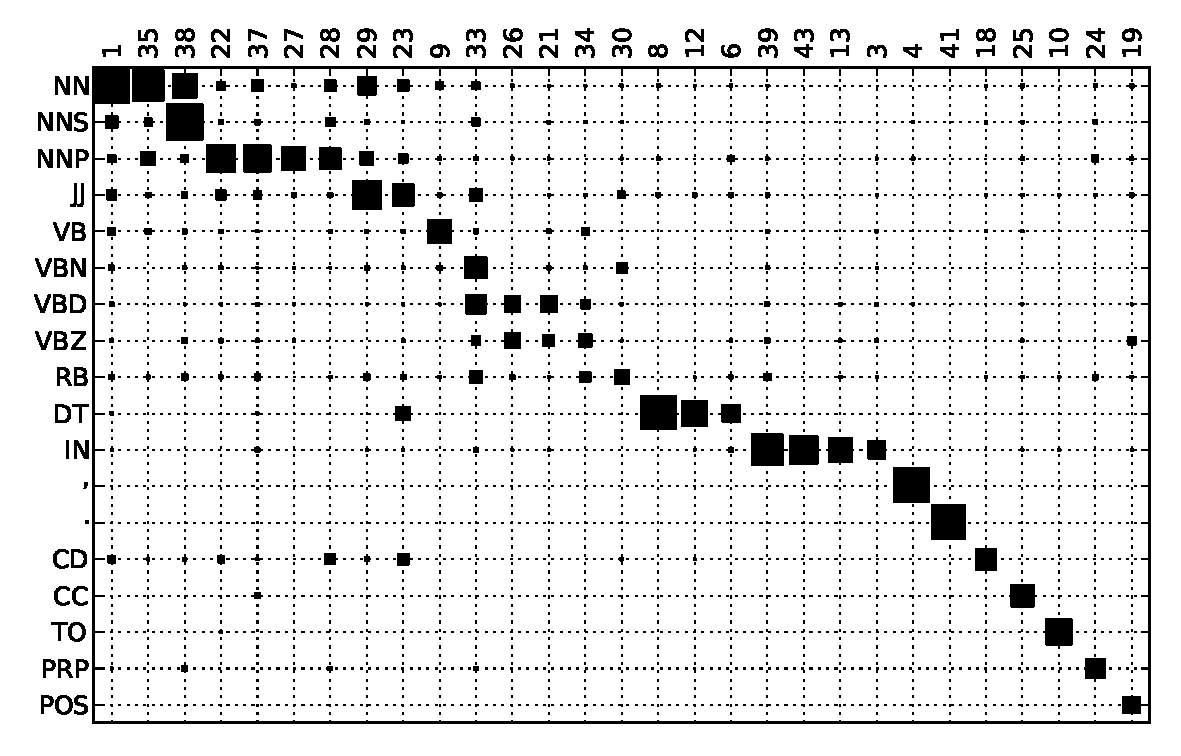
\includegraphics[width=\textwidth]{hinton.eps}
\vspace*{-10mm}
\caption{Hinton diagram of the most frequent tags (rows) and clusters
  (columns).  Area of each square is proportional to the joint
  probability of the given tag and cluster.}
\label{fig:hinton}
\end{figure*}

\section{Discussion}
\label{sec:discussion}

Figure~\ref{fig:hinton} is the Hinton diagram showing the relationship
between the most frequent tags and clusters found by the collapsed
algorithm (\collapseResult\% many-to-one accuracy).  In this section
we present a qualitative comparison of gold standard tags and
discovered clusters.

\paragraph{Nouns and adjectives:} Most nouns ({\sc nn*}) are split between the
clusters represented by the first seven columns of the Hinton graph,
but not in the way Penn Treebank splits them.  For example cluster 27
brings together titles like {\em Mr.}, {\em Mrs.}, {\em Dr.}
etc. which does not exist as a separate class in the gold tags.
Cluster 29 is the largest adjective ({\sc jj}) cluster, however it
also has noun members probably due to the difficulty of separating
noun-noun compounds and adjective modification.

\paragraph{Verbs and adverbs:}  Clusters 9 and 33 contain general
verbs ({\sc vb*}), but the verbs ``be'' (26), ``say'' (21), and
``have'' (34) have been split into their own clusters indicated in
parantheses, presumably because they are not generally substitutable
with the rest.  Adverb ({\sc rb}) is an amorphous class and the
algorithm seems to have difficulty isolating it in a cluster.

\paragraph{Determiners and prepositions:}  We see a fairly clean
separation of determiners ({\sc dt}) and prepositions ({\sc in}) from
other parts of speech, although each has been subdivided into further
groups by the algorithm.  For example cluster 39 contains general
prepositions but ``of'' (43), ``in'' (13), and ``for'' (3) are split
into their own clusters.  Determiners ``the'' (8), ``a'' (12), and
capitalized ``The''/''A'' (6) are also split into their own clusters.

\paragraph{Closed-class items:}  Most closed-class items are cleanly
separated into their own clusters as seen in the lower right hand
corner of the diagram.

\section{Contributions}
\label{sec:contrib}

We introduced a paradigmatic representation for word context which
contains possible substitutes for the target word and their
probabilities.  The substitute probabilities were estimated using a
standard 4-gram language model with Kneser-Ney smoothing.  We
investigated distance metrics, dimensionality reduction techniques and
clustering algorithms appropriate for substitute probability vectors
and evaluated them using a supervised k-nearest-neighbor baseline and
many-to-one accuracy relative to a 45-tag 24K word test corpus.  We
found that the KL2 distance metric (a symmetric version of
Kullback-Leibler divergence), dimensionality reduction using Laplacian
eigenmaps, and spectral clustering work well with substitute vectors.
Spectral clustering of substitute vectors reveal a grouping that
largely match traditional part of speech boundaries (\spectralResult\%
many-to-one accuracy) which further improve when the one-tag-per-word
constraint is imposed (\collapseResult\% many-to-one accuracy).  These
results compare favorably to previous results published for the 45-tag
24K word test corpus we have used.  
%% We are investigating ways to speed up the algorithm so it can be tested on larger corpora.

\bibliographystyle{acl2012}
\bibliography{posind2012}

\end{document}
